% Gráficos generados a partir de las respuestas de la encuesta (n = 16).
\begin{figure}[htbp]
\centering
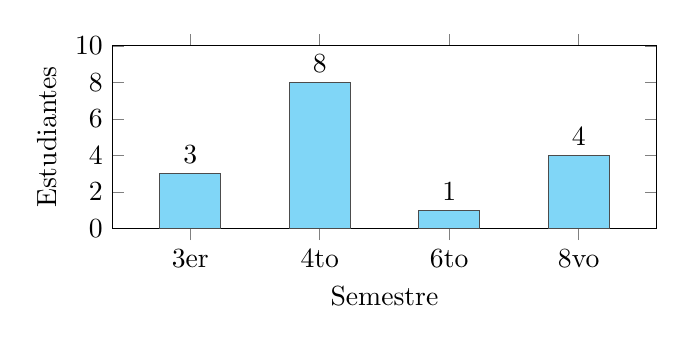
\begin{tikzpicture}
\begin{axis}[ybar, bar width=22pt, width=0.7\textwidth, height=3.9cm, ymin=0, ymax=10,
    ylabel={Estudiantes}, xlabel={Semestre}, symbolic x coords={3er,4to,6to,8vo}, xtick=data,
    nodes near coords, enlarge x limits=0.2]
\addplot[fill=cyan!50, draw=black!70] coordinates {(3er,3) (4to,8) (6to,1) (8vo,4)};
\end{axis}
\end{tikzpicture}
\caption{Nivel de avance de los estudiantes encuestados.}
\label{fig:enc_nivel}
\elaboradopor{\autorTFG}
\fuente{Respuestas al cuestionario del Anexo~B ($n = 16$)}
\end{figure}

\begin{figure}[htbp]
\centering
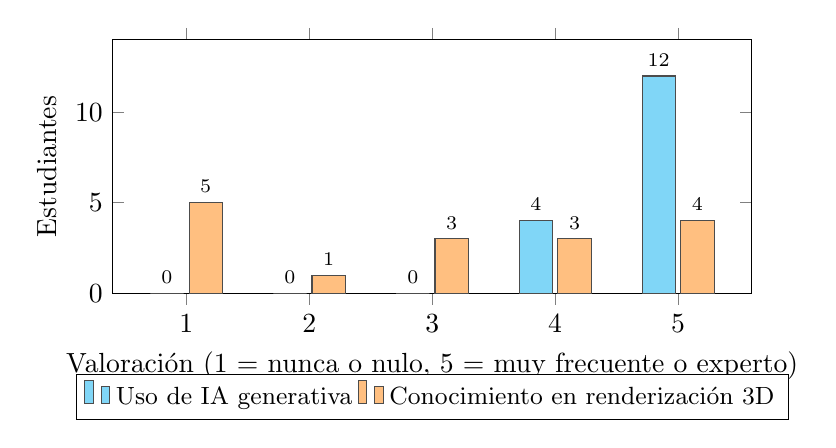
\begin{tikzpicture}
\begin{axis}[ybar, bar width=12pt, width=0.8\textwidth, height=4.8cm, ymin=0, ymax=14,
    ylabel={Estudiantes}, xlabel={Valoración (1 = nunca o nulo, 5 = muy frecuente o experto)}, xtick={1,2,3,4,5},
    nodes near coords, nodes near coords style={font=\scriptsize}, enlarge x limits=0.15,
    legend style={at={(0.5,-0.32)}, anchor=north, legend columns=2, font=\small}]
\addplot[fill=cyan!50, draw=black!70] coordinates {(1,0) (2,0) (3,0) (4,4) (5,12)};
\addplot[fill=orange!50, draw=black!70] coordinates {(1,5) (2,1) (3,3) (4,3) (5,4)};
\legend{Uso de IA generativa, Conocimiento en renderización 3D}
\end{axis}
\end{tikzpicture}
\caption{Uso previo de IA generativa y conocimiento técnico en renderización 3D.}
\elaboradopor{\autorTFG}
\fuente{Respuestas al cuestionario del Anexo~B ($n = 16$)}
\end{figure}

\begin{figure}[htbp]
\centering
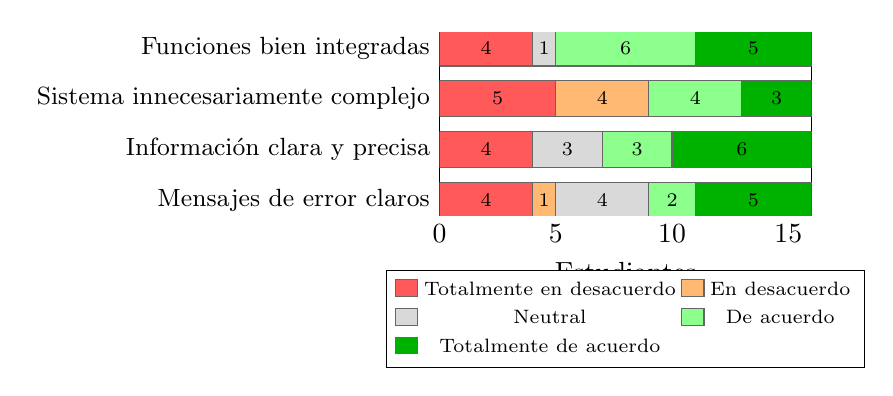
\begin{tikzpicture}
\begin{axis}[xbar stacked, bar width=13pt, width=0.52\textwidth, height=3.9cm,
    xmin=0, xmax=16, xlabel={Estudiantes}, symbolic y coords={Funciones bien integradas,Sistema innecesariamente complejo,Información clara y precisa,Mensajes de error claros}, ytick=data,
    y tick label style={font=\small}, y dir=reverse,
    point meta=rawx,
    nodes near coords={\pgfmathfloatifflags{\pgfplotspointmeta}{0}{}{\pgfmathprintnumber{\pgfplotspointmeta}}},
    nodes near coords style={font=\scriptsize},
    legend style={at={(0.5,-0.3)}, anchor=north, legend columns=2, font=\scriptsize}]
\addplot[fill=red!65, draw=black!60] coordinates {(4,Funciones bien integradas) (5,Sistema innecesariamente complejo) (4,Información clara y precisa) (4,Mensajes de error claros)};
\addplot[fill=orange!55, draw=black!60] coordinates {(0,Funciones bien integradas) (4,Sistema innecesariamente complejo) (0,Información clara y precisa) (1,Mensajes de error claros)};
\addplot[fill=gray!30, draw=black!60] coordinates {(1,Funciones bien integradas) (0,Sistema innecesariamente complejo) (3,Información clara y precisa) (4,Mensajes de error claros)};
\addplot[fill=green!45, draw=black!60] coordinates {(6,Funciones bien integradas) (4,Sistema innecesariamente complejo) (3,Información clara y precisa) (2,Mensajes de error claros)};
\addplot[fill=green!70!black, draw=black!60] coordinates {(5,Funciones bien integradas) (3,Sistema innecesariamente complejo) (6,Información clara y precisa) (5,Mensajes de error claros)};
\legend{Totalmente en desacuerdo,En desacuerdo,Neutral,De acuerdo,Totalmente de acuerdo}
\end{axis}
\end{tikzpicture}
\caption{Usabilidad de la interfaz: integración, complejidad (ítem inverso), claridad y mensajes de error.}
\elaboradopor{\autorTFG}
\fuente{Respuestas al cuestionario del Anexo~B ($n = 16$)}
\end{figure}

\begin{figure}[htbp]
\centering
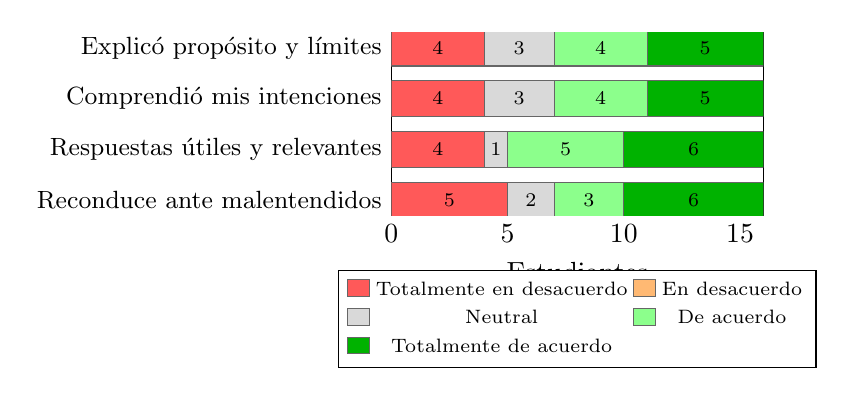
\begin{tikzpicture}
\begin{axis}[xbar stacked, bar width=13pt, width=0.52\textwidth, height=3.9cm,
    xmin=0, xmax=16, xlabel={Estudiantes}, symbolic y coords={Explicó propósito y límites,Comprendió mis intenciones,Respuestas útiles y relevantes,Reconduce ante malentendidos}, ytick=data,
    y tick label style={font=\small}, y dir=reverse,
    point meta=rawx,
    nodes near coords={\pgfmathfloatifflags{\pgfplotspointmeta}{0}{}{\pgfmathprintnumber{\pgfplotspointmeta}}},
    nodes near coords style={font=\scriptsize},
    legend style={at={(0.5,-0.3)}, anchor=north, legend columns=2, font=\scriptsize}]
\addplot[fill=red!65, draw=black!60] coordinates {(4,Explicó propósito y límites) (4,Comprendió mis intenciones) (4,Respuestas útiles y relevantes) (5,Reconduce ante malentendidos)};
\addplot[fill=orange!55, draw=black!60] coordinates {(0,Explicó propósito y límites) (0,Comprendió mis intenciones) (0,Respuestas útiles y relevantes) (0,Reconduce ante malentendidos)};
\addplot[fill=gray!30, draw=black!60] coordinates {(3,Explicó propósito y límites) (3,Comprendió mis intenciones) (1,Respuestas útiles y relevantes) (2,Reconduce ante malentendidos)};
\addplot[fill=green!45, draw=black!60] coordinates {(4,Explicó propósito y límites) (4,Comprendió mis intenciones) (5,Respuestas útiles y relevantes) (3,Reconduce ante malentendidos)};
\addplot[fill=green!70!black, draw=black!60] coordinates {(5,Explicó propósito y límites) (5,Comprendió mis intenciones) (6,Respuestas útiles y relevantes) (6,Reconduce ante malentendidos)};
\legend{Totalmente en desacuerdo,En desacuerdo,Neutral,De acuerdo,Totalmente de acuerdo}
\end{axis}
\end{tikzpicture}
\caption{Inteligencia conversacional: propósito, comprensión, utilidad y reconducción.}
\elaboradopor{\autorTFG}
\fuente{Respuestas al cuestionario del Anexo~B ($n = 16$)}
\end{figure}

\begin{figure}[htbp]
\centering
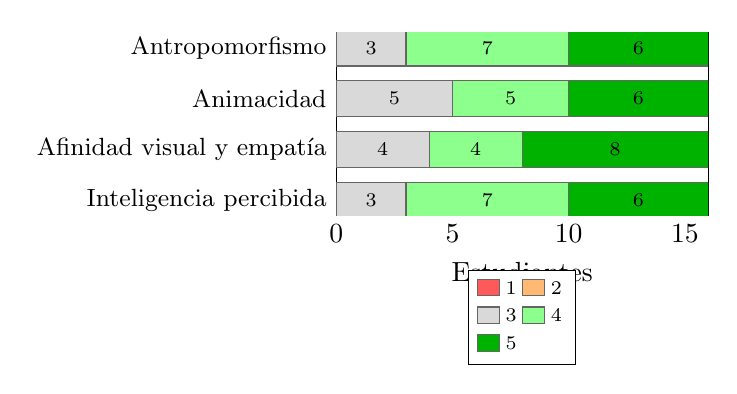
\begin{tikzpicture}
\begin{axis}[xbar stacked, bar width=13pt, width=0.52\textwidth, height=3.9cm,
    xmin=0, xmax=16, xlabel={Estudiantes}, symbolic y coords={Antropomorfismo,Animacidad,Afinidad visual y empatía,Inteligencia percibida}, ytick=data,
    y tick label style={font=\small}, y dir=reverse,
    point meta=rawx,
    nodes near coords={\pgfmathfloatifflags{\pgfplotspointmeta}{0}{}{\pgfmathprintnumber{\pgfplotspointmeta}}},
    nodes near coords style={font=\scriptsize},
    legend style={at={(0.5,-0.3)}, anchor=north, legend columns=2, font=\scriptsize}]
\addplot[fill=red!65, draw=black!60] coordinates {(0,Antropomorfismo) (0,Animacidad) (0,Afinidad visual y empatía) (0,Inteligencia percibida)};
\addplot[fill=orange!55, draw=black!60] coordinates {(0,Antropomorfismo) (0,Animacidad) (0,Afinidad visual y empatía) (0,Inteligencia percibida)};
\addplot[fill=gray!30, draw=black!60] coordinates {(3,Antropomorfismo) (5,Animacidad) (4,Afinidad visual y empatía) (3,Inteligencia percibida)};
\addplot[fill=green!45, draw=black!60] coordinates {(7,Antropomorfismo) (5,Animacidad) (4,Afinidad visual y empatía) (7,Inteligencia percibida)};
\addplot[fill=green!70!black, draw=black!60] coordinates {(6,Antropomorfismo) (6,Animacidad) (8,Afinidad visual y empatía) (6,Inteligencia percibida)};
\legend{1,2,3,4,5}
\end{axis}
\end{tikzpicture}
\caption{Percepción del avatar 3D en el diferencial semántico (1 a 5).}
\label{fig:enc_avatar}
\elaboradopor{\autorTFG}
\fuente{Respuestas al cuestionario del Anexo~B ($n = 16$)}
\end{figure}

\begin{figure}[htbp]
\centering
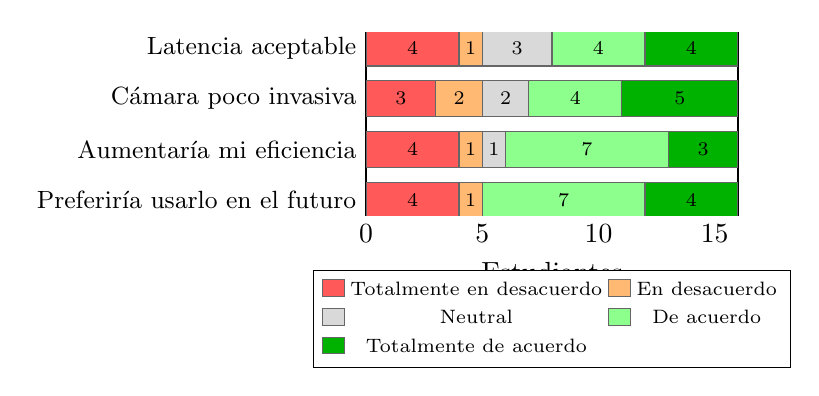
\begin{tikzpicture}
\begin{axis}[xbar stacked, bar width=13pt, width=0.52\textwidth, height=3.9cm,
    xmin=0, xmax=16, xlabel={Estudiantes}, symbolic y coords={Latencia aceptable,Cámara poco invasiva,Aumentaría mi eficiencia,Preferiría usarlo en el futuro}, ytick=data,
    y tick label style={font=\small}, y dir=reverse,
    point meta=rawx,
    nodes near coords={\pgfmathfloatifflags{\pgfplotspointmeta}{0}{}{\pgfmathprintnumber{\pgfplotspointmeta}}},
    nodes near coords style={font=\scriptsize},
    legend style={at={(0.5,-0.3)}, anchor=north, legend columns=2, font=\scriptsize}]
\addplot[fill=red!65, draw=black!60] coordinates {(4,Latencia aceptable) (3,Cámara poco invasiva) (4,Aumentaría mi eficiencia) (4,Preferiría usarlo en el futuro)};
\addplot[fill=orange!55, draw=black!60] coordinates {(1,Latencia aceptable) (2,Cámara poco invasiva) (1,Aumentaría mi eficiencia) (1,Preferiría usarlo en el futuro)};
\addplot[fill=gray!30, draw=black!60] coordinates {(3,Latencia aceptable) (2,Cámara poco invasiva) (1,Aumentaría mi eficiencia) (0,Preferiría usarlo en el futuro)};
\addplot[fill=green!45, draw=black!60] coordinates {(4,Latencia aceptable) (4,Cámara poco invasiva) (7,Aumentaría mi eficiencia) (7,Preferiría usarlo en el futuro)};
\addplot[fill=green!70!black, draw=black!60] coordinates {(4,Latencia aceptable) (5,Cámara poco invasiva) (3,Aumentaría mi eficiencia) (4,Preferiría usarlo en el futuro)};
\legend{Totalmente en desacuerdo,En desacuerdo,Neutral,De acuerdo,Totalmente de acuerdo}
\end{axis}
\end{tikzpicture}
\caption{Aceptación tecnológica: latencia, uso de la cámara, eficiencia y preferencia futura.}
\label{fig:enc_aceptacion}
\elaboradopor{\autorTFG}
\fuente{Respuestas al cuestionario del Anexo~B ($n = 16$)}
\end{figure}
